\documentclass[11pt, A4paper, english]{article}
\usepackage{amsfonts}
\usepackage{amsmath}
\usepackage{amssymb}
\usepackage{amsthm}
\usepackage{babel}
\usepackage{color}
\usepackage{float}
\usepackage[T1]{fontenc}
\usepackage{graphicx}
\usepackage[colorlinks]{hyperref}
\usepackage[utf8]{inputenc}
\usepackage{listings}
\usepackage{textcomp}
\usepackage[style=ieee]{biblatex}
\usepackage{tabularx}
\usepackage{multicol}

\addbibresource{bibliography.bib}

\definecolor{url}{rgb}{0.1, 0.1, 0.4}

\lstset{frame=tb,
	language=csh,
	aboveskip=3mm,
	belowskip=3mm,
	showstringspaces=false,
	columns=flexible,
	basicstyle={\small\ttfamily},
	numbers=none,
	breaklines=true,
	breakatwhitespace=true,
	tabsize=3
}

\lstset{inputpath="C:/Users/Torstein/Documents/skole/USN/IIA2017/Assignment 6"}
\graphicspath{{C:/Users/Torstein/Documents/USN/IIA2017/Assignment 6/}}
\hypersetup{colorlinks = true, linkcolor = black, urlcolor=url}

\author{Torstein Solheim Ølberg | 263054 \\
	University of South-Eastern Norway}
\title{SCADA System for Air Heater}



%\lstinputlisting{Filnavn! type kodefil}. Use [linerange=0-73] or [linerange=73-] to crop
%\includegraphics[width=12.6cm, height=8cm]{Filnavn! type png}



\begin{document}
	\maketitle
	
	\begin{multicols}{2}
		\section{Abstract}
\textbf{Keyword:} \textit{SCADA, LabVIEW, WindowsForms, Simulation}

		\section{Introduction}
During the winter of 2024, the residents of Landskronaveien 49 experienced that their heating system was unable to keep up with the fall in temperature. As a result, a new air heater system must be installed, adding to the system already in effect. This system must be capable of heating the air, measuring the temperature of the environment and alert the residents if the temperature is outside the comfortable range. For this purpose, a SCADA (supervisory control and data acquisition) system has been chose and the general structure of the product can be seen if figure \ref{system_sketch}. As the hardware for the system has not arrived yet, a simulating setup of the system was produced. Only a single heater simulator, controller and server is possible to begin with due to this shortage in hardware, but this can easily be expanded upon later. \\
			\begin{figure}[H]
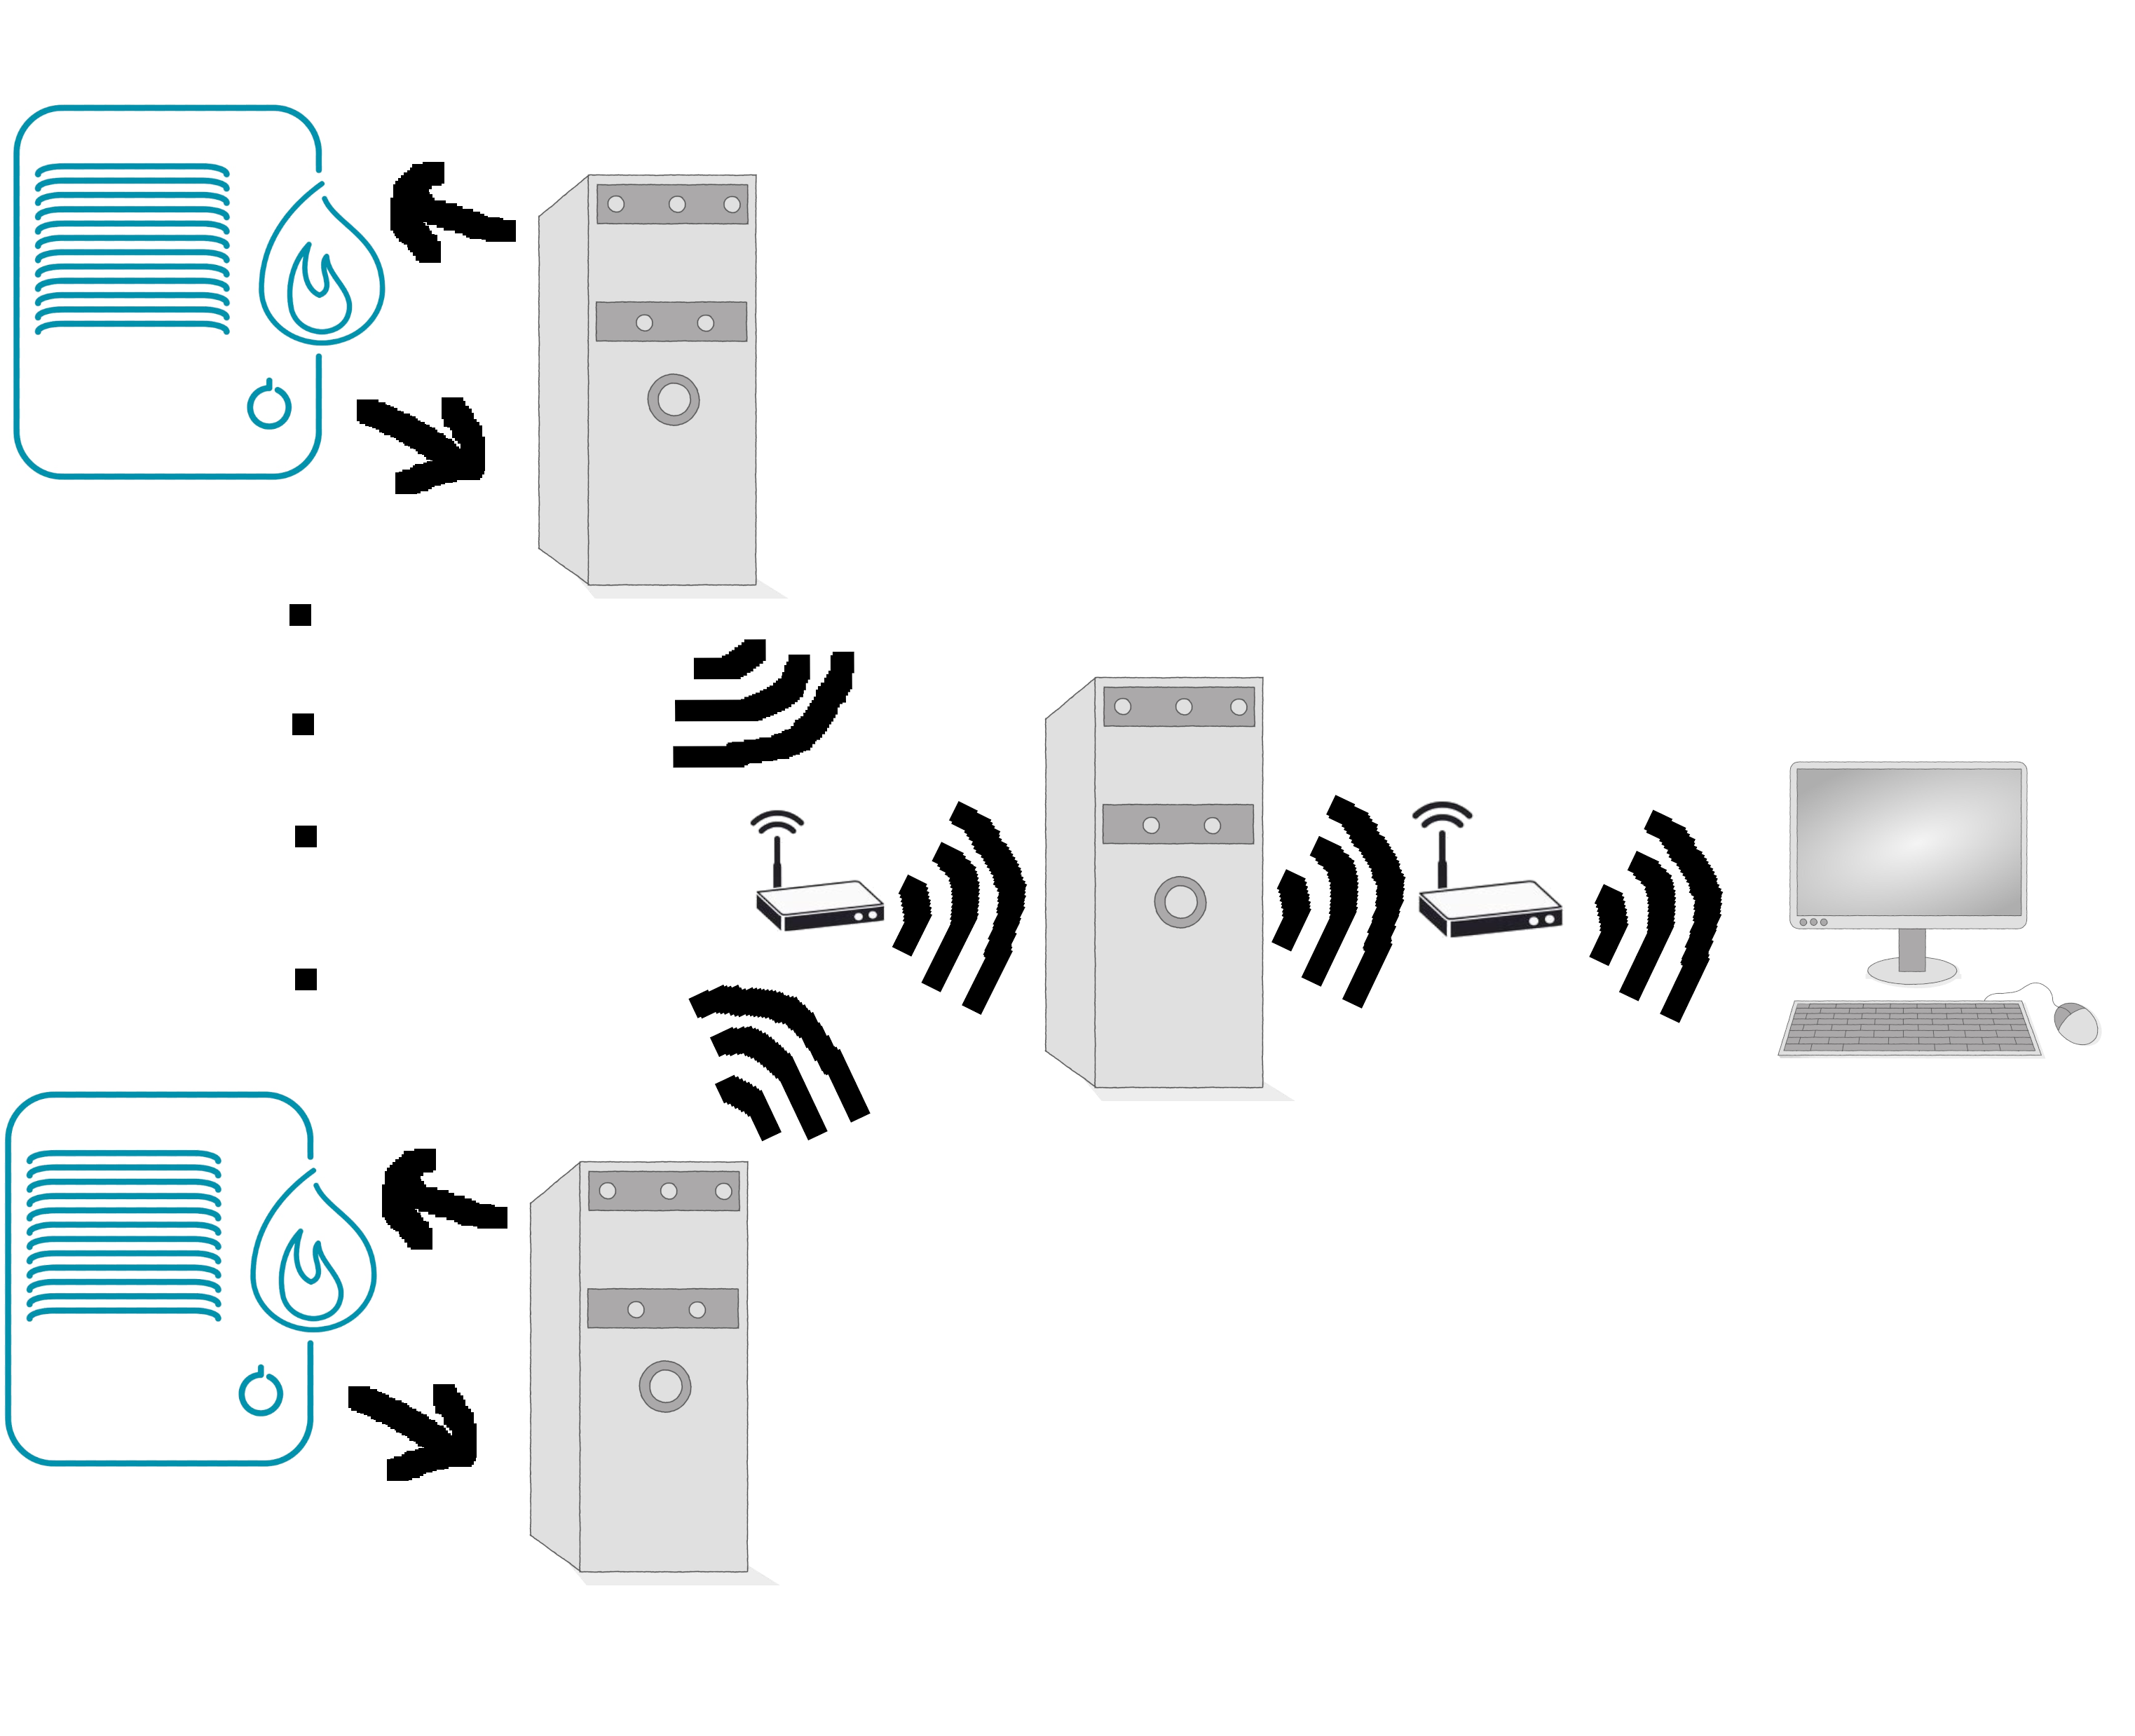
\includegraphics[width=\columnwidth]{SCADA_sketch.png}
\caption{SCADA system sketch.}
\label{system_sketch}
			\end{figure}
This report will outline the process which was done to create this system. First, the methods and tools used to develop the system will be presented. Then, the system will be presented, along with the most important parts of the code and the results of testing it. Finally, the usefulness of the system and its capability to solve the problem will be discussed and a conclusion will be drawn.
		
		
		\section{Materials and Methods}
The Method section will outline the tools and methods used for development of the system. Each subsection will present a different set of tools and how they where used in this project.
		
		\subsection{Airheater}
The heater which has been ordered for use in the system is the same one presented by Haugen \cite{airheater}. It consists of a fan which sucks in air, a heater controller taking in an electric signal between zero and five volt, and a temperature sensor which gives of a one to five volt electrical signal corresponding to between zero and 50 degrees Celsius. Since this heater is not available yet, a simulated heater model \cite{airheatermodel} has ben used instead. This airheater model 
		
		\subsection{LabVIEW}
		
		
		\subsection{Controller}
		
		
		\subsection{OPC UA Server}
		
		
		\subsection{SQL Server}
		
		
		\subsection{Visual Studio, C#, WindowsForms and The Display Application}
		
		\section{Results}
		
		
		\section{Discussion}
This section discusses the system with regard to its fulfilment of the original specification and any future improvements upon the work.
		
		
		\section{Conclusion}
		
		
\printbibliography
		
	\end{multicols}
\end{document}
